% ----------------------------------------------------------------------
%
%                            TFMTesis.tex
%
%----------------------------------------------------------------------
%
% Este fichero contiene el "documento maestro" del documento. Lo único
% que hace es configurar el entorno LaTeX e incluir los ficheros .tex
% que contienen cada sección.
%
%----------------------------------------------------------------------
%
% Los ficheros necesarios para este documento son:
%
%       TeXiS/* : ficheros de la plantilla TeXiS.
%       Cascaras/* : ficheros con las partes del documento que no
%          son capítulos ni apéndices (portada, agradecimientos, etc.)
%       Capitulos/*.tex : capítulos de la tesis
%       Apendices/*.tex: apéndices de la tesis
%       constantes.tex: constantes LaTeX
%       config.tex : configuración de la "compilación" del documento
%       guionado.tex : palabras con guiones
%
% Para la bibliografía, además, se necesitan:
%
%       *.bib : ficheros con la información de las referencias
%
% ---------------------------------------------------------------------

\documentclass[11pt,a4paper,twoside]{book}

%
% Definimos  el   comando  \compilaCapitulo,  que   luego  se  utiliza
% (opcionalmente) en config.tex. Quedaría  mejor si también se definiera
% en  ese fichero,  pero por  el modo  en el  que funciona  eso  no es
% posible. Puedes consultar la documentación de ese fichero para tener
% más  información. Definimos también  \compilaApendice, que  tiene el
% mismo  cometido, pero  que se  utiliza para  compilar  únicamente un
% apéndice.
%
%
% Si  queremos   compilar  solo   una  parte  del   documento  podemos
% especificar mediante  \includeonly{...} qué ficheros  son los únicos
% que queremos  que se incluyan.  Esto  es útil por  ejemplo para sólo
% compilar un capítulo.
%
% El problema es que todos aquellos  ficheros que NO estén en la lista
% NO   se  incluirán...  y   eso  también   afecta  a   ficheros  de
% la plantilla...
%
% Total,  que definimos  una constante  con los  ficheros  que siempre
% vamos a querer compilar  (aquellos relacionados con configuración) y
% luego definimos \compilaCapitulo.
\newcommand{\ficherosBasicosTeXiS}{%
TeXiS/TeXiS_pream,TeXiS/TeXiS_cab,TeXiS/TeXiS_bib,TeXiS/TeXiS_cover%
}
\newcommand{\ficherosBasicosTexto}{%
constantes,guionado,Cascaras/bibliografia,config%
}
\newcommand{\compilaCapitulo}[1]{%
\includeonly{\ficherosBasicosTeXiS,\ficherosBasicosTexto,Capitulos/#1}%
}

\newcommand{\compilaApendice}[1]{%
\includeonly{\ficherosBasicosTeXiS,\ficherosBasicosTexto,Apendices/#1}%
}

%- - - - - - - - - - - - - - - - - - - - - - - - - - - - - - - - - - -
%            Preámbulo del documento. Configuraciones varias
%- - - - - - - - - - - - - - - - - - - - - - - - - - - - - - - - - - -

% Define  el  tipo  de  compilación que  estamos  haciendo.   Contiene
% definiciones  de  constantes que  cambian  el  comportamiento de  la
% compilación. Debe incluirse antes del paquete TeXiS/TeXiS.sty
%---------------------------------------------------------------------
%
%                          config.tex
%
%---------------------------------------------------------------------
%
% Contiene la  definición de constantes  que determinan el modo  en el
% que se compilará el documento.
%
%---------------------------------------------------------------------
%
% En concreto, podemos  indicar si queremos "modo release",  en el que
% no  aparecerán  los  comentarios  (creados  mediante  \com{Texto}  o
% \comp{Texto}) ni los "por  hacer" (creados mediante \todo{Texto}), y
% sí aparecerán los índices. El modo "debug" (o mejor dicho en modo no
% "release" muestra los índices  (construirlos lleva tiempo y son poco
% útiles  salvo  para   la  versión  final),  pero  sí   el  resto  de
% anotaciones.
%
% Si se compila con LaTeX (no  con pdflatex) en modo Debug, también se
% muestran en una esquina de cada página las entradas (en el índice de
% palabras) que referencian  a dicha página (consulta TeXiS_pream.tex,
% en la parte referente a show).
%
% El soporte para  el índice de palabras en  TeXiS es embrionario, por
% lo  que no  asumas que  esto funcionará  correctamente.  Consulta la
% documentación al respecto en TeXiS_pream.tex.
%
%
% También  aquí configuramos  si queremos  o  no que  se incluyan  los
% acrónimos  en el  documento final  en la  versión release.  Para eso
% define (o no) la constante \acronimosEnRelease.
%
% Utilizando \compilaCapitulo{nombre}  podemos también especificar qué
% capítulo(s) queremos que se compilen. Si no se pone nada, se compila
% el documento  completo.  Si se pone, por  ejemplo, 01Introduccion se
% compilará únicamente el fichero Capitulos/01Introduccion.tex
%
% Para compilar varios  capítulos, se separan sus nombres  con comas y
% no se ponen espacios de separación.
%
% En realidad  la macro \compilaCapitulo  está definida en  el fichero
% principal tesis.tex.
%
%---------------------------------------------------------------------


% Comentar la línea si no se compila en modo release.
% TeXiS hará el resto.
% ¡¡¡Si cambias esto, haz un make clean antes de recompilar!!!
\def\release{1}


% Descomentar la linea si se quieren incluir los
% acrónimos en modo release (en modo debug
% no se incluirán nunca).
% ¡¡¡Si cambias esto, haz un make clean antes de recompilar!!!
%\def\acronimosEnRelease{1}


% Descomentar la línea para establecer el capítulo que queremos
% compilar

% \compilaCapitulo{01Introduccion}
% \compilaCapitulo{02EstructuraYGeneracion}
% \compilaCapitulo{03Edicion}
% \compilaCapitulo{04Imagenes}
% \compilaCapitulo{05Bibliografia}
% \compilaCapitulo{06Makefile}

% \compilaApendice{01AsiSeHizo}

% Variable local para emacs, para  que encuentre el fichero maestro de
% compilación y funcionen mejor algunas teclas rápidas de AucTeX
%%%
%%% Local Variables:
%%% mode: latex
%%% TeX-master: "./Tesis.tex"
%%% End:


% Paquete de la plantilla
\usepackage{TeXiS/TeXiS}
\usepackage{graphicx}

% Incluimos el fichero con comandos de constantes
%---------------------------------------------------------------------
%
%                          constantes.tex
%
%---------------------------------------------------------------------
%
% Fichero que  declara nuevos comandos LaTeX  sencillos realizados por
% comodidad en la escritura de determinadas palabras
%
%---------------------------------------------------------------------

%%%%%%%%%%%%%%%%%%%%%%%%%%%%%%%%%%%%%%%%%%%%%%%%%%%%%%%%%%%%%%%%%%%%%%
% Comando: 
%
%       \titulo
%
% Resultado: 
%
% Escribe el título del documento.
%%%%%%%%%%%%%%%%%%%%%%%%%%%%%%%%%%%%%%%%%%%%%%%%%%%%%%%%%%%%%%%%%%%%%%
\def\titulo{\textsc{TeXiS}: Sistema de intercambio de archivos P2P}

%%%%%%%%%%%%%%%%%%%%%%%%%%%%%%%%%%%%%%%%%%%%%%%%%%%%%%%%%%%%%%%%%%%%%%
% Comando: 
%
%       \autor
%
% Resultado: 
%
% Escribe el autor del documento.
%%%%%%%%%%%%%%%%%%%%%%%%%%%%%%%%%%%%%%%%%%%%%%%%%%%%%%%%%%%%%%%%%%%%%%
\def\autor{Sergio Garc\'ia S\'anchez}

% Variable local para emacs, para  que encuentre el fichero maestro de
% compilación y funcionen mejor algunas teclas rápidas de AucTeX

%%%
%%% Local Variables:
%%% mode: latex
%%% TeX-master: "tesis.tex"
%%% End:


% Sacamos en el log de la compilación el copyright
%\typeout{Copyright Marco Antonio and Pedro Pablo Gomez Martin}

%
% "Metadatos" para el PDF
%
\ifpdf\hypersetup{%
    pdftitle = {\titulo},
    pdfsubject = {Plantilla de Tesis},
    pdfkeywords = {Plantilla, LaTeX, tesis, trabajo de
      investigación, trabajo de Master},
    pdfauthor = {\textcopyright\ \autor},
    pdfcreator = {\LaTeX\ con el paquete \flqq hyperref\frqq},
    pdfproducer = {pdfeTeX-0.\the\pdftexversion\pdftexrevision},
    }
    \pdfinfo{/CreationDate (\today)}
\fi


%- - - - - - - - - - - - - - - - - - - - - - - - - - - - - - - - - - -
%                        Documento
%- - - - - - - - - - - - - - - - - - - - - - - - - - - - - - - - - - -
\begin{document}

% Incluimos el  fichero de definición de guionado  de algunas palabras
% que LaTeX no ha dividido como debería
%----------------------------------------------------------------
%
%                          guionado.tex
%
%----------------------------------------------------------------
%
% Fichero con algunas divisiones de palabras que LaTeX no
% hace correctamente si no se le da alguna ayuda.
%
%----------------------------------------------------------------

\hyphenation{
% a
abs-trac-to
abs-trac-tos
abs-trac-ta
abs-trac-tas
ac-tua-do-res
a-gra-de-ci-mien-tos
ana-li-za-dor
an-te-rio-res
an-te-rior-men-te
apa-rien-cia
a-pro-pia-do
a-pro-pia-dos
a-pro-pia-da
a-pro-pia-das
a-pro-ve-cha-mien-to
a-que-llo
a-que-llos
a-que-lla
a-que-llas
a-sig-na-tu-ra
a-sig-na-tu-ras
a-so-cia-da
a-so-cia-das
a-so-cia-do
a-so-cia-dos
au-to-ma-ti-za-do
% b
batch
bi-blio-gra-fía
bi-blio-grá-fi-cas
bien
bo-rra-dor
boo-l-ean-expr
% c
ca-be-ce-ra
call-me-thod-ins-truc-tion
cas-te-lla-no
cir-cuns-tan-cia
cir-cuns-tan-cias
co-he-ren-te
co-he-ren-tes
co-he-ren-cia
co-li-bri
co-men-ta-rio
co-mer-cia-les
co-no-ci-mien-to
cons-cien-te
con-si-de-ra-ba
con-si-de-ra-mos
con-si-de-rar-se
cons-tan-te
cons-trucción
cons-tru-ye
cons-tru-ir-se
con-tro-le
co-rrec-ta-men-te
co-rres-pon-den
co-rres-pon-dien-te
co-rres-pon-dien-tes
co-ti-dia-na
co-ti-dia-no
crean
cris-ta-li-zan
cu-rri-cu-la
cu-rri-cu-lum
cu-rri-cu-lar
cu-rri-cu-la-res
% d
de-di-ca-do
de-di-ca-dos
de-di-ca-da
de-di-ca-das
de-rro-te-ro
de-rro-te-ros
de-sa-rro-llo
de-sa-rro-llos
de-sa-rro-lla-do
de-sa-rro-lla-dos
de-sa-rro-lla-da
de-sa-rro-lla-das
de-sa-rro-lla-dor
de-sa-rro-llar
des-cri-bi-re-mos
des-crip-ción
des-crip-cio-nes
des-cri-to
des-pués
de-ta-lla-do
de-ta-lla-dos
de-ta-lla-da
de-ta-lla-das
di-a-gra-ma
di-a-gra-mas
di-se-ños
dis-po-ner
dis-po-ni-bi-li-dad
do-cu-men-ta-da
do-cu-men-to
do-cu-men-tos
% e
edi-ta-do
e-du-ca-ti-vo
e-du-ca-ti-vos
e-du-ca-ti-va
e-du-ca-ti-vas
e-la-bo-ra-do
e-la-bo-ra-dos
e-la-bo-ra-da
e-la-bo-ra-das
es-co-llo
es-co-llos
es-tu-dia-do
es-tu-dia-dos
es-tu-dia-da
es-tu-dia-das
es-tu-dian-te
e-va-lua-cio-nes
e-va-lua-do-res
exis-ten-tes
exhaus-ti-va
ex-pe-rien-cia
ex-pe-rien-cias
% f
for-ma-li-za-do
% g
ge-ne-ra-ción
ge-ne-ra-dor
ge-ne-ra-do-res
ge-ne-ran
% h
he-rra-mien-ta
he-rra-mien-tas
% i
i-dio-ma
i-dio-mas
im-pres-cin-di-ble
im-pres-cin-di-bles
in-de-xa-do
in-de-xa-dos
in-de-xa-da
in-de-xa-das
in-di-vi-dual
in-fe-ren-cia
in-fe-ren-cias
in-for-ma-ti-ca
in-gre-dien-te
in-gre-dien-tes
in-me-dia-ta-men-te
ins-ta-la-do
ins-tan-cias
% j
% k
% l
len-gua-je
li-be-ra-to-rio
li-be-ra-to-rios
li-be-ra-to-ria
li-be-ra-to-rias
li-mi-ta-do
li-te-ra-rio
li-te-ra-rios
li-te-ra-ria
li-te-ra-rias
lo-tes
% m
ma-ne-ra
ma-nual
mas-que-ra-de
ma-yor
me-mo-ria
mi-nis-te-rio
mi-nis-te-rios
mo-de-lo
mo-de-los
mo-de-la-do
mo-du-la-ri-dad
mo-vi-mien-to
% n
na-tu-ral
ni-vel
nues-tro
% o
obs-tan-te
o-rien-ta-do
o-rien-ta-dos
o-rien-ta-da
o-rien-ta-das
% p
pa-ra-le-lo
pa-ra-le-la
par-ti-cu-lar
par-ti-cu-lar-men-te
pe-da-gó-gi-ca
pe-da-gó-gi-cas
pe-da-gó-gi-co
pe-da-gó-gi-cos
pe-rio-di-ci-dad
per-so-na-je
plan-te-a-mien-to
plan-te-a-mien-tos
po-si-ción
pre-fe-ren-cia
pre-fe-ren-cias
pres-cin-di-ble
pres-cin-di-bles
pri-me-ra
pro-ble-ma
pro-ble-mas
pró-xi-mo
pu-bli-ca-cio-nes
pu-bli-ca-do
% q
% r
rá-pi-da
rá-pi-do
ra-zo-na-mien-to
ra-zo-na-mien-tos
re-a-li-zan-do
re-fe-ren-cia
re-fe-ren-cias
re-fe-ren-cia-da
re-fe-ren-cian
re-le-van-tes
re-pre-sen-ta-do
re-pre-sen-ta-dos
re-pre-sen-ta-da
re-pre-sen-ta-das
re-pre-sen-tar-lo
re-qui-si-to
re-qui-si-tos
res-pon-der
res-pon-sa-ble
% s
se-pa-ra-do
si-guien-do
si-guien-te
si-guien-tes
si-guie-ron
si-mi-lar
si-mi-la-res
si-tua-ción
% t
tem-pe-ra-ments
te-ner
trans-fe-ren-cia
trans-fe-ren-cias
% u
u-sua-rio
Unreal-Ed
% v
va-lor
va-lo-res
va-rian-te
ver-da-de-ro
ver-da-de-ros
ver-da-de-ra
ver-da-de-ras
ver-da-de-ra-men-te
ve-ri-fi-ca
% w
% x
% y
% z
}
% Variable local para emacs, para que encuentre el fichero
% maestro de compilación
%%%
%%% Local Variables:
%%% mode: latex
%%% TeX-master: "./Tesis.tex"
%%% End:


% Marcamos  el inicio  del  documento para  la  numeración de  páginas
% (usando números romanos para esta primera fase).
\frontmatter
\pagestyle{empty}

%---------------------------------------------------------------------
%
%                          configCover.tex
%
%---------------------------------------------------------------------
%
% cover.tex
% Copyright 2009 Marco Antonio Gomez-Martin, Pedro Pablo Gomez-Martin
%
% This file belongs to the TeXiS manual, a LaTeX template for writting
% Thesis and other documents. The complete last TeXiS package can
% be obtained from http://gaia.fdi.ucm.es/projects/texis/
%
% Although the TeXiS template itself is distributed under the 
% conditions of the LaTeX Project Public License
% (http://www.latex-project.org/lppl.txt), the manual content
% uses the CC-BY-SA license that stays that you are free:
%
%    - to share & to copy, distribute and transmit the work
%    - to remix and to adapt the work
%
% under the following conditions:
%
%    - Attribution: you must attribute the work in the manner
%      specified by the author or licensor (but not in any way that
%      suggests that they endorse you or your use of the work).
%    - Share Alike: if you alter, transform, or build upon this
%      work, you may distribute the resulting work only under the
%      same, similar or a compatible license.
%
% The complete license is available in
% http://creativecommons.org/licenses/by-sa/3.0/legalcode
%
%---------------------------------------------------------------------
%
% Fichero que contiene la configuración de la portada y de la 
% primera hoja del documento.
%
%---------------------------------------------------------------------


% Pueden configurarse todos los elementos del contenido de la portada
% utilizando comandos.

%%%%%%%%%%%%%%%%%%%%%%%%%%%%%%%%%%%%%%%%%%%%%%%%%%%%%%%%%%%%%%%%%%%%%%
% Título del documento:
% \tituloPortada{titulo}
% Nota:
% Si no se define se utiliza el del \titulo. Este comando permite
% cambiar el título de forma que se especifiquen dónde se quieren
% los retornos de carro cuando se utilizan fuentes grandes.
%%%%%%%%%%%%%%%%%%%%%%%%%%%%%%%%%%%%%%%%%%%%%%%%%%%%%%%%%%%%%%%%%%%%%%
\tituloPortada{%
Sistema de intercambio de archivos P2P
}


%%%%%%%%%%%%%%%%%%%%%%%%%%%%%%%%%%%%%%%%%%%%%%%%%%%%%%%%%%%%%%%%%%%%%%
% Título del documento en inglés:
% \tituloPortadaEng{titulo}
% Nota:
% Si no se define se utiliza el del \titulo. Este comando permite
% cambiar el título de forma que se especifiquen dónde se quieren
% los retornos de carro cuando se utilizan fuentes grandes.
%%%%%%%%%%%%%%%%%%%%%%%%%%%%%%%%%%%%%%%%%%%%%%%%%%%%%%%%%%%%%%%%%%%%%%
\tituloPortadaEng{%
P2P File Sharing System"
}

%%%%%%%%%%%%%%%%%%%%%%%%%%%%%%%%%%%%%%%%%%%%%%%%%%%%%%%%%%%%%%%%%%%%%%
% Autor del documento:
% \autorPortada{Nombre}
% Se utiliza en la portada y en el valor por defecto del
% primer subtítulo de la segunda portada.
%%%%%%%%%%%%%%%%%%%%%%%%%%%%%%%%%%%%%%%%%%%%%%%%%%%%%%%%%%%%%%%%%%%%%%
\autorPortada{Sergio Garc\'ia S\'anchez}

%%%%%%%%%%%%%%%%%%%%%%%%%%%%%%%%%%%%%%%%%%%%%%%%%%%%%%%%%%%%%%%%%%%%%%
% Fecha de publicación:
% \fechaPublicacion{Fecha}
% Puede ser vacío. Aparece en la última línea de ambas portadas
%%%%%%%%%%%%%%%%%%%%%%%%%%%%%%%%%%%%%%%%%%%%%%%%%%%%%%%%%%%%%%%%%%%%%%
% Descomentar para que ponga siempre la fecha actual
%\fechaPublicacion{\today}
\fechaPublicacion{\textcolor{red}{DIA de MES de AÑO}}

%%%%%%%%%%%%%%%%%%%%%%%%%%%%%%%%%%%%%%%%%%%%%%%%%%%%%%%%%%%%%%%%%%%%%%
% Imagen de la portada (y escala)
% \imagenPortada{Fichero}
% \escalaImagenPortada{Numero}
% Si no se especifica, se utiliza la imagen TODO.pdf
%%%%%%%%%%%%%%%%%%%%%%%%%%%%%%%%%%%%%%%%%%%%%%%%%%%%%%%%%%%%%%%%%%%%%%
% imagen en blanco y negro
%\imagenPortada{Imagenes/Vectorial/escudoUCM}
%imagen en color
\imagenPortada{Imagenes/Bitmap/escudoUCMcolor}
\escalaImagenPortada{.2}

%%%%%%%%%%%%%%%%%%%%%%%%%%%%%%%%%%%%%%%%%%%%%%%%%%%%%%%%%%%%%%%%%%%%%%
% Tipo de documento.
% \tipoDocumento{Tipo}
% Para el texto justo debajo del escudo.
% Si no se indica, se utiliza "TESIS DOCTORAL".
%%%%%%%%%%%%%%%%%%%%%%%%%%%%%%%%%%%%%%%%%%%%%%%%%%%%%%%%%%%%%%%%%%%%%%
\tipoDocumento{Trabajo de Fin de Máster}

%%%%%%%%%%%%%%%%%%%%%%%%%%%%%%%%%%%%%%%%%%%%%%%%%%%%%%%%%%%%%%%%%%%%%%
% Institución/departamento asociado al documento.
% \institucion{Nombre}
% Puede tener varias líneas. Se utiliza en las dos portadas.
% Si no se indica aparecerá vacío.
%%%%%%%%%%%%%%%%%%%%%%%%%%%%%%%%%%%%%%%%%%%%%%%%%%%%%%%%%%%%%%%%%%%%%%
\institucion{%
Máster en Ingeniería Informática\\[0.2em]
Facultad de Informática\\[0.2em]
Universidad Complutense de Madrid
}

%%%%%%%%%%%%%%%%%%%%%%%%%%%%%%%%%%%%%%%%%%%%%%%%%%%%%%%%%%%%%%%%%%%%%%
% Director del trabajo.
% \directorPortada{Nombre}
% Se utiliza para el valor por defecto del segundo subtítulo, donde
% se indica quién es el director del trabajo.
% Si se fuerza un subtítulo distinto, no hace falta definirlo.
%%%%%%%%%%%%%%%%%%%%%%%%%%%%%%%%%%%%%%%%%%%%%%%%%%%%%%%%%%%%%%%%%%%%%%
\directorPortada{Adri\'an Riesco Rodr\'iguez}



%%%%%%%%%%%%%%%%%%%%%%%%%%%%%%%%%%%%%%%%%%%%%%%%%%%%%%%%%%%%%%%%%%%%%%
% Texto del primer subtítulo de la segunda portada.
% \textoPrimerSubtituloPortada{Texto}
% Para configurar el primer "texto libre" de la segunda portada.
% Si no se especifica se indica "Memoria que presenta para optar al
% título de Doctor en Informática" seguido del \autorPortada.
%%%%%%%%%%%%%%%%%%%%%%%%%%%%%%%%%%%%%%%%%%%%%%%%%%%%%%%%%%%%%%%%%%%%%%
\textoPrimerSubtituloPortada{%
\textbf{Trabajo de Fin de Máster en Ingeniería Informática}  \\ [0.3em]
\textbf{Departamento de \textcolor{red}{XXXXXXXXXXXXX}} \\ [0.3em]
}

%%%%%%%%%%%%%%%%%%%%%%%%%%%%%%%%%%%%%%%%%%%%%%%%%%%%%%%%%%%%%%%%%%%%%%
% Texto del segundo subtítulo de la segunda portada.
% \textoSegundoSubtituloPortada{Texto}
% Para configurar el segundo "texto libre" de la segunda portada.
% Si no se especifica se indica "Dirigida por el Doctor" seguido
% del \directorPortada.
%%%%%%%%%%%%%%%%%%%%%%%%%%%%%%%%%%%%%%%%%%%%%%%%%%%%%%%%%%%%%%%%%%%%%%
\textoSegundoSubtituloPortada{%
\textbf{Convocatoria: }\textit{\textcolor{red}{Febrero/Junio/Septiembre} \the\year} \\ [0.2em]
\textbf{Calificación: }\textit{\textcolor{red}{Nota}}
}

%%%%%%%%%%%%%%%%%%%%%%%%%%%%%%%%%%%%%%%%%%%%%%%%%%%%%%%%%%%%%%%%%%%%%%
% \explicacionDobleCara
% Si se utiliza, se aclara que el documento está preparado para la
% impresión a doble cara.
%%%%%%%%%%%%%%%%%%%%%%%%%%%%%%%%%%%%%%%%%%%%%%%%%%%%%%%%%%%%%%%%%%%%%%
%\explicacionDobleCara

%%%%%%%%%%%%%%%%%%%%%%%%%%%%%%%%%%%%%%%%%%%%%%%%%%%%%%%%%%%%%%%%%%%%%%
% \isbn
% Si se utiliza, aparecerá el ISBN detrás de la segunda portada.
%%%%%%%%%%%%%%%%%%%%%%%%%%%%%%%%%%%%%%%%%%%%%%%%%%%%%%%%%%%%%%%%%%%%%%
%\isbn{978-84-692-7109-4}


%%%%%%%%%%%%%%%%%%%%%%%%%%%%%%%%%%%%%%%%%%%%%%%%%%%%%%%%%%%%%%%%%%%%%%
% \copyrightInfo
% Si se utiliza, aparecerá información de los derechos de copyright
% detrás de la segunda portada.
%%%%%%%%%%%%%%%%%%%%%%%%%%%%%%%%%%%%%%%%%%%%%%%%%%%%%%%%%%%%%%%%%%%%%%
%\copyrightInfo{\autor}


%%
%% Creamos las portadas
%%
\makeCover

% Variable local para emacs, para que encuentre el fichero
% maestro de compilación
%%%
%%% Local Variables:
%%% mode: latex
%%% TeX-master: "../Tesis.tex"
%%% End:

%\chapter*{Autorización de difusión}

   
El abajo firmante, matriculado en el Máster en Ingeniería en Informática de la Facultad de Informática, autoriza a la Universidad Complutense de Madrid (UCM) a difundir y utilizar con fines académicos, no comerciales y mencionando expresamente a su autor el presente Trabajo Fin de Máster: ``TITULO DEL TRABAJO'', realizado durante el curso académico CURSO bajo la dirección de DIRECTORES en el Departamento de XXXXXXXXXXXXXXXXXXXXXXXX, y a la Biblioteca de la UCM a depositarlo en el Archivo Institucional E-Prints Complutense con el objeto de incrementar la difusión, uso e impacto del trabajo en Internet y garantizar su preservación y acceso a largo plazo.

\vspace{5cm}

% +--------------------------------------------------------------------+
% | On the line below, replace "Enter Your Name" with your name
% | Use the same form of your name as it appears on your title page.
% | Use mixed case, for example, Lori Goetsch.
% +--------------------------------------------------------------------+
\begin{center}
	\large Nombre Del Alumno\\
	
	\vspace{0.5cm}
	
	% +--------------------------------------------------------------------+
	% | On the line below, replace Fecha
	% |
	% +--------------------------------------------------------------------+
	
	\today\\
	
\end{center}

% +--------------------------------------------------------------------+
% | Dedication Page (Optional)
% +--------------------------------------------------------------------+

\chapter*{Dedicatoria}

\begin{flushright}
\begin{minipage}[c]{8.5cm}
\flushright{\textit{A Pedro Pablo y Marco Antonio, por crear TeXiS e iluminar nuestro camino}}
\end{minipage}
\end{flushright}
% +--------------------------------------------------------------------+
% | Acknowledgements Page (Optional)                                   |
% +--------------------------------------------------------------------+

\chapter*{Agradecimientos}

A Guillermo, por el tiempo empleado en hacer estas plantillas. A Adrián, Enrique y Nacho, por sus comentarios para mejorar lo que hicimos. Y a Narciso, a quien no le ha hecho falta el Anillo Único para coordinarnos a todos.












\chapter*{Resumen}

\section*{\tituloPortadaVal}

Un resumen en castellano de media página, incluyendo el título en castellano. A continuación, se escribirá una lista de no más de 10 palabras clave.


\section*{Palabras clave}
   
\noindent Máximo 10 palabras clave separadas por comas

   



\begin{otherlanguage}{english}
\chapter*{Abstract}

\section*{\tituloPortadaEngVal}

An abstract in English, half a page long, including the title in English. Below, a list with no more than 10 keywords.


\section*{Keywords}

\noindent 10 keywords max., separated by commas.




% Si el trabajo se escribe en inglés, comentar esta línea y descomentar
% otra igual que hay justo antes de \end{document}
\end{otherlanguage}

\ifx\generatoc\undefined
\else
%---------------------------------------------------------------------
%
%                          TeXiS_toc.tex
%
%---------------------------------------------------------------------
%
% TeXiS_toc.tex
% Copyright 2009 Marco Antonio Gomez-Martin, Pedro Pablo Gomez-Martin
%
% This file belongs to TeXiS, a LaTeX template for writting
% Thesis and other documents. The complete last TeXiS package can
% be obtained from http://gaia.fdi.ucm.es/projects/texis/
%
% This work may be distributed and/or modified under the
% conditions of the LaTeX Project Public License, either version 1.3
% of this license or (at your option) any later version.
% The latest version of this license is in
%   http://www.latex-project.org/lppl.txt
% and version 1.3 or later is part of all distributions of LaTeX
% version 2005/12/01 or later.
%
% This work has the LPPL maintenance status `maintained'.
% 
% The Current Maintainers of this work are Marco Antonio Gomez-Martin
% and Pedro Pablo Gomez-Martin
%
%---------------------------------------------------------------------
%
% Contiene  los  comandos  para  generar los  índices  del  documento,
% entendiendo por índices las tablas de contenidos.
%
% Genera  el  índice normal  ("tabla  de  contenidos"),  el índice  de
% figuras y el de tablas. También  crea "marcadores" en el caso de que
% se esté compilando con pdflatex para que aparezcan en el PDF.
%
%---------------------------------------------------------------------


% Primero un poquito de configuración...


% Pedimos que inserte todos los epígrafes hasta el nivel \subsection en
% la tabla de contenidos.
\setcounter{tocdepth}{2} 

% Le  pedimos  que nos  numere  todos  los  epígrafes hasta  el  nivel
% \subsubsection en el cuerpo del documento.
\setcounter{secnumdepth}{3} 


% Creamos los diferentes índices.

% Lo primero un  poco de trabajo en los marcadores  del PDF. No quiero
% que  salga una  entrada  por cada  índice  a nivel  0...  si no  que
% aparezca un marcador "Índices", que  tenga dentro los otros tipos de
% índices.  Total, que creamos el marcador "Índices".
% Antes de  la creación  de los índices,  se añaden los  marcadores de
% nivel 1.

\ifpdf
   \pdfbookmark{Índices}{indices}
\fi

% Tabla de contenidos.
%
% La  inclusión  de '\tableofcontents'  significa  que  en la  primera
% pasada  de  LaTeX  se  crea   un  fichero  con  extensión  .toc  con
% información sobre la tabla de contenidos (es conceptualmente similar
% al  .bbl de  BibTeX, creo).  En la  segunda ejecución  de  LaTeX ese
% documento se utiliza para  generar la verdadera página de contenidos
% usando la  información sobre los  capítulos y demás guardadas  en el
% .toc
\ifpdf
   \pdfbookmark[1]{Tabla de Contenidos}{tabla de contenidos}
\fi

\cabeceraEspecial{\'Indice}

\tableofcontents

\newpage 

% Índice de figuras
%
% La idea es semejante que para  el .toc del índice, pero ahora se usa
% extensión .lof (List Of Figures) con la información de las figuras.

\ifpdf
   \pdfbookmark[1]{Índice de figuras}{indice de figuras}
\fi

\cabeceraEspecial{\'Indice de figuras}

\listoffigures

\newpage

% Índice de tablas
% Como antes, pero ahora .lot (List Of Tables)

\ifpdf
   \pdfbookmark[1]{Índice de tablas}{indice de tablas}
\fi

\cabeceraEspecial{\'Indice de tablas}

\listoftables

\newpage

% Variable local para emacs, para  que encuentre el fichero maestro de
% compilación y funcionen mejor algunas teclas rápidas de AucTeX

%%%
%%% Local Variables:
%%% mode: latex
%%% TeX-master: "../Tesis.tex"
%%% End:

\fi

% Marcamos el  comienzo de  los capítulos (para  la numeración  de las
% páginas) y ponemos la cabecera normal
\mainmatter

\pagestyle{fancy}
\restauraCabecera


\chapter{Introducción}
\label{cap:introduccion}


\section{Contexto}

Las redes Peer-to-Peer (P2P) representan un modelo de comunicación descentralizado en el que todos los nodos participan de forma equitativa, actuando tanto como clientes como servidores.
Este paradigma, alternativo al modelo cliente-servidor tradicional, ha transformado la forma en que compartimos información y utilizamos los recursos en línea.
Su impacto ha sido especialmente notable en el ámbito del intercambio de archivos,
donde su capacidad para distribuir grandes volúmenes de datos sin depender de servidores centralizados ha supuesto una revolución tecnológica \cite{schollmeier2001}.


\begin{figure}[h]
    \centering
    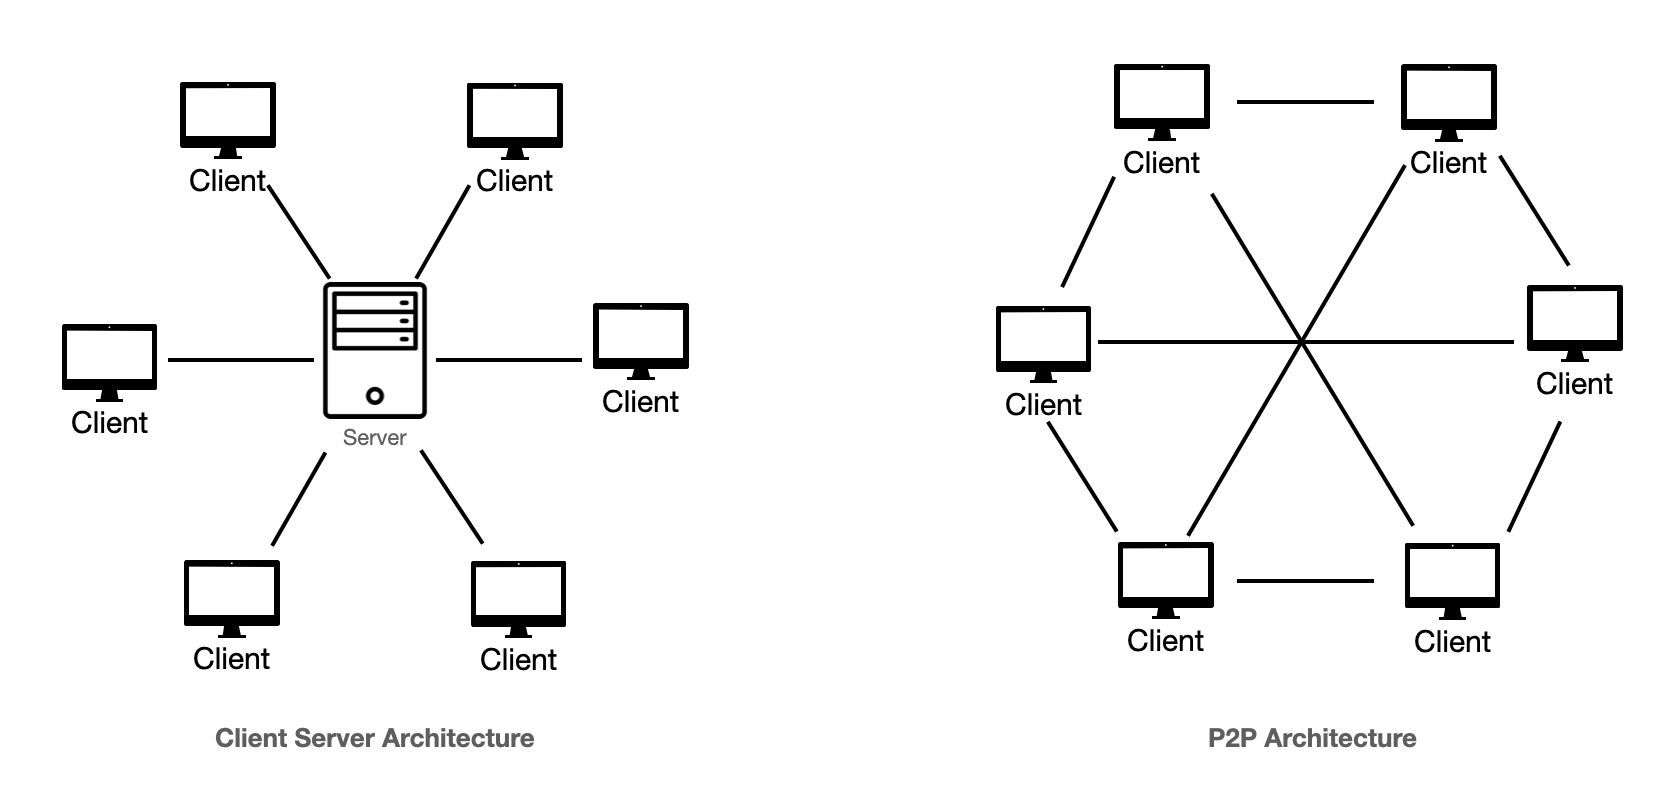
\includegraphics[width = 0.5\textwidth]{Imagenes/Vectorial/client-server-vs-p2p}
    \caption{Comparaci\'on entre arquitectura cliente-servidor y arquitectura P2P}
    \label{fig:clientVsp2p}
\end{figure}


El inicio de las redes P2P modernas se remonta a finales de la década de 1990, con la aparición de Napster en 1999.
Napster introdujo un modelo centralizado en el que los usuarios podían buscar y descargar archivos, principalmente música, a través de un servidor que indexaba todos los contenidos disponibles.
Esta plataforma, aunque técnicamente no era completamente P2P debido a su dependencia de un servidor central,
fue pionera en popularizar el intercambio de archivos entre pares.


Sin embargo, Napster enfrentó múltiples desafíos legales, principalmente por el intercambio no autorizado de material protegido por derechos de autor.
Estos problemas llevaron a su cierre en 2001, pero también impulsaron el desarrollo de alternativas más descentralizadas que no dependían de un punto único de control.


La caída de Napster marcó el comienzo de una segunda generación de redes P2P, más resilientes y descentralizadas.
Plataformas como Gnutella y eDonkey surgieron como respuesta a la vulnerabilidad inherente de los sistemas centralizados.
Gnutella, por ejemplo, permitió que cada nodo en la red actuara de forma completamente independiente, eliminando la necesidad de un servidor central.


Estas redes introdujeron nuevos retos técnicos, como la búsqueda eficiente de archivos en una red distribuida y el manejo de grandes volúmenes de tráfico.
Para abordar estos problemas, se desarrollaron algoritmos más avanzados para la localización de recursos y técnicas de segmentación de archivos para optimizar la transferencia de datos.


La llegada de BitTorrent en 2001 marcó un nuevo hito en la evolución de las redes P2P.
Este protocolo introdujo un enfoque innovador para el intercambio de archivos al dividirlos en fragmentos más pequeños. L
os usuarios podían descargar estos fragmentos desde múltiples fuentes simultáneamente, lo que mejoraba significativamente la velocidad y la eficiencia de las transferencias.
Además, BitTorrent redujo la carga sobre los nodos individuales al permitir que los usuarios que habían descargado partes de un archivo las compartieran inmediatamente con otros \cite{cohen2003}.


A lo largo de los años, las redes P2P han evolucionado para abarcar aplicaciones más allá del intercambio de archivos.
En la actualidad, estas tecnologías son fundamentales en áreas como el streaming de vídeo, los juegos en línea y, más recientemente, las plataformas basadas en blockchain como Bitcoin.
Este último caso destaca por su capacidad para descentralizar no solo la transferencia de datos, sino también el control financiero, mediante un registro distribuido y seguro.



\section{Motivación}

Las redes Peer-to-Peer (P2P) han transformado la manera en que compartimos información y utilizamos recursos en línea,
posicionándose como una alternativa eficiente y escalable al modelo cliente-servidor.
A pesar de su relevancia y aplicaciones actuales en campos como el intercambio de archivos, el streaming de vídeo y las plataformas blockchain,
el diseño e implementación de estas redes desde un nivel práctico sigue siendo un reto para muchos desarrolladores.

Este trabajo no busca competir con las grandes plataformas que emplean arquitecturas P2P ni desarrollar una red masiva con millones de usuarios.
En cambio, se enfoca en la creación de una red P2P funcional desde cero, con énfasis en los conceptos fundamentales y su implementación práctica.

Con ello, se espera facilitar el entendimiento de este modelo descentralizado y motivar el desarrollo de nuevas aplicaciones basadas en redes P2P,
adaptadas a los desafíos tecnológicos contemporáneos.


\section{Objetivos}

El objetivo principal de este trabajo es diseñar e implementar una red Peer-to-Peer (P2P) funcional para el intercambio de archivos de manera distribuida,
integrando tecnologías actuales como UPnP para la gestión automática de puertos y un sistema centralizado para la localización y conexión de nodos.
Este desarrollo se centrará en la creación de un cliente con interfaz gráfica que sirva como base para todas las funcionalidades de la red.

Para alcanzar este objetivo general, se plantean los siguientes objetivos específicos:

\begin{itemize}
    \item \textbf{Desarrollar un cliente con interfaz gráfica:} Diseñar e implementar una aplicación gráfica que permita a los usuarios compartir y descargar archivos de manera sencilla e intuitiva. Este cliente será el núcleo sobre el cual se integrarán las funcionalidades de la red P2P.

    \item \textbf{Desarrollar un sistema de registro y gestión de nodos:} Implementar un mecanismo centralizado que permita identificar y coordinar los peers conectados a la red, facilitando su interacción y comunicación.

    \item \textbf{Diseñar e implementar la comunicación directa entre nodos:} Crear un protocolo basado en TCP que permita a los peers establecer conexiones fiables y seguras para el intercambio de archivos, asegurando una comunicación robusta y compatible con redes distribuidas.

    \item \textbf{Integrar soporte para UPnP:} Automatizar la configuración de puertos en los routers mediante el uso de UPnP, garantizando una conectividad sencilla y accesible para los usuarios.

    \item \textbf{Implementar un sistema de intercambio de archivos distribuido:} Diseñar un modelo que permita a los peers compartir y descargar archivos fragmentados desde múltiples fuentes, optimizando el uso de los recursos de la red.

    \item \textbf{Documentar el diseño, implementación y evaluación del sistema:} Elaborar una descripción técnica detallada del desarrollo de la red P2P, incluyendo los algoritmos y tecnologías utilizadas, así como las

\end{itemize}


\section{Plan de trabajo}

Durante el desarrollo del proyecto se ha seguido un plan de trabajo detallado con el objetivo de estructurar las tareas y garantizar el cumplimiento de los objetivos planteados. La planificación ha permitido organizar de forma eficiente las distintas fases del desarrollo, estableciendo prioridades y tiempos. El plan de trabajo se ha dividido en los siguientes puntos:

\begin{enumerate}

    \item \textbf{Estudio de las tecnologías a utilizar:}
    Se llevó a cabo un análisis detallado de las tecnologías necesarias para el desarrollo del proyecto, incluyendo protocolos de comunicación como TCP,
    sistemas de apertura de puertos con UPnP y arquitecturas P2P para el intercambio de archivos.
    Este estudio incluyó la búsqueda de documentación técnica, recursos en línea y herramientas que facilitaran el desarrollo.

    \item \textbf{Desarrollo del cliente con interfaz gráfica:}
    Se inició el diseño e implementación en java del cliente gráfico como base del proyecto.
    Este cliente incluye funcionalidades esenciales para compartir y descargar archivos, sirviendo como núcleo sobre el cual se desarrollaron las demás características de la red.
    Durante esta fase, se probaron aspectos básicos de la interacción con el sistema de archivos local.

    \item \textbf{Implementación del sistema de registro de nodos:}
    Se diseñó e implementó un sistema centralizado para gestionar los nodos conectados a la red.
    Este sistema permite registrar los peers activos y facilitar su descubrimiento entre ellos.
    Además, se integró con el cliente para garantizar que los usuarios pudieran conectarse a otros peers de manera eficiente.

    \item \textbf{Diseño e implementación de la comunicación entre nodos:}
    Se desarrolló un protocolo basado en TCP para la conexión directa entre peers.
    Esta etapa incluyó pruebas para garantizar la fiabilidad y estabilidad de las conexiones, así como su integración con el cliente gráfico.

    \item \textbf{Integración del soporte para UPnP:}
    Se implementó soporte para la configuración automática de puertos mediante UPnP, lo que permitió facilitar la conexión entre nodos en redes con configuraciones complejas,
    eliminando la necesidad de ajustes manuales por parte del usuario.

    \item \textbf{Evaluación y pruebas del sistema:}
    Se llevaron a cabo pruebas funcionales para verificar el correcto funcionamiento de cada componente de la red P2P, así como su integración global.
    Estas pruebas incluyeron casos con múltiples nodos conectados para garantizar la robustez del sistema.

    \item \textbf{Escritura y revisión de la memoria:}
    Durante las fases de implementación y pruebas, se elaboró la memoria del proyecto, documentando las decisiones tomadas, los resultados obtenidos y los aprendizajes adquiridos.

    \item \textbf{Cierre del proyecto:}
    Una vez terminadas todas las fases, se realizó una revisión final del cliente y de la memoria, realizando las correcciones necesarias para su entrega final.
    Se verificó que todos los objetivos se hubieran cumplido satisfactoriamente antes del cierre del proyecto.
\end{enumerate}

En definitiva, un plan de trabajo bien estructurado ha permitido avanzar de manera eficiente y cumplir con los hitos establecidos dentro del tiempo límite.

\chapter{Fundamentos t\'eoricos}
\label{cap:fundamentosTeoricos}

Este capítulo aborda los fundamentos teóricos necesarios para comprender las redes Peer-to-Peer (P2P), comenzando con su definición y evolución histórica.
También, se analizan los tipos de arquitecturas P2P más comunes y los distintos protocolos que permiten su funcionamiento, como TCP y UPnP.

\section{Introducción a las redes P2P}
Las redes P2P son sistemas de comunicación que se caracterizan por su arquitectura descentralizada, donde todos los nodos de la red desempeñan roles equivalentes.
Esto significa que los nodos actúan tanto como clientes, solicitando recursos, como servidores, compartiendo datos con otros nodos.
Según \cite{schollmeier2001}, una red P2P se define por su capacidad para que los nodos compartan recursos directamente entre ellos, sin depender de una entidad central que coordine o gestione las interacciones.
Este enfoque fomenta la resiliencia y la escalabilidad, ya que la red no depende de un único punto de fallo.

En contraste, el modelo cliente-servidor tradicional se basa en un servidor central que almacena los datos y responde a las solicitudes de los clientes.
Este modelo tiene algunas limitaciones importantes, como posibles cuellos de botella y la vulnerabilidad a fallos del servidor centralizado \cite{coulouris2011}.
Por el contrario, las redes P2P distribuyen la carga de trabajo entre todos los nodos, aprovechando la capacidad colectiva de la red para manejar grandes volúmenes de datos de manera eficiente.

\paragraph{Primera generación de redes P2P}

El desarrollo moderno de las redes P2P comenzó en 1999 con la aparición de Napster, una plataforma diseñada para compartir música.
Napster marcó un hito al permitir que los usuarios intercambiaran archivos directamente, popularizando el concepto de redes P2P \cite{oram2001}.
Su arquitectura introdujo el uso de servidores para indexar recursos, una tecnología que facilitaba la búsqueda y transferencia de archivos.
Sin embargo, su dependencia de un único punto de control lo convirtió en un objetivo legal vulnerable.
El cierre de Napster en 2001 marcó el final de esta primera etapa y el inicio de redes P2P más descentralizadas.

\paragraph{Segunda generación de redes P2P}

La segunda generación de redes P2P, representada por plataformas como Gnutella y eDonkey, eliminó los servidores centrales y adoptó modelos completamente distribuidos.
En Gnutella, por ejemplo, cada nodo se conectaba directamente con otros nodos vecinos, formando una red en malla.
Aunque esta descentralización mejoró la resiliencia de la red, también introdujo grandes retos técnicos.
Entre los principales desafíos se encontraban la búsqueda eficiente de recursos en una red distribuida y la gestión del tráfico generado por los distintos nodos \cite{risson2006}.

Por su parte, eDonkey introdujo mejoras en la forma de localizar archivos, empleando servidores auxiliares para agilizar las búsquedas, pero manteniendo la transferencia directa entre nodos.
Estas plataformas demostraron que las redes P2P podían escalar y manejar grandes cantidades de datos, pero también dejaron claro la necesidad de mejorar su funcionamiento.

\paragraph{BitTorrent y la fragmentación de archivos}

En 2001, BitTorrent marcó un punto de inflexión en la evolución de las redes P2P al introducir un nuevo enfoque para el intercambio de archivos.
En lugar de que un nodo descargara un archivo completo de otro, BitTorrent dividía los archivos en fragmentos más pequeños.
Esto permitía que un usuario descargara diferentes fragmentos de un archivo desde múltiples nodos simultáneamente, aumentando la eficiencia del ancho de banda disponible \cite{cohen2003}.
Además, los nodos comenzaban a compartir los fragmentos descargados con otros usuarios antes de completar la descarga, lo que aumentaba la colaboración entre los nodos.

Esta innovación convirtió a BitTorrent en una tecnología líder en el intercambio de archivos y popularizó el uso de las redes P2P entre los usuarios,
demostrando su capacidad para manejar grandes volúmenes de datos de manera eficiente.

\paragraph{Relevancia actual de las redes P2P}

En la actualidad, las redes P2P van más alla del ámbito del intercambio de archivos y se han adaptado a una amplia gama de aplicaciones.
Por ejemplo, en el streaming de contenido, tecnologías como WebRTC aprovechan la conectividad directa entre nodos para mejorar la latencia y reducir la carga en servidores centrales.
Además, plataformas basadas en blockchain, como Bitcoin, utilizan redes P2P para garantizar la descentralización no solo en la transferencia de datos, sino también en la gestión financiera.
Según \cite{nakamoto2008}, la arquitectura P2P es fundamental para el funcionamiento de Bitcoin, ya que elimina la necesidad de intermediarios y permite un sistema financiero más transparente y seguro.

\section{Arquitecturas de redes P2P}

La arquitectura de una red P2P define cómo los nodos se organizan para compartir recursos y comunicarse entre ellos.
Este aspecto estructural tiene un gran impacto en la eficiencia, escalabilidad y resiliencia de la red.
Existen tres tipos principales de arquitecturas en redes P2P: centralizadas, descentralizadas e híbridas \cite{schollmeier2001, risson2006}.

\subsection{Arquitecturas centralizadas}

Las arquitecturas centralizadas en redes P2P se caracterizan por la presencia de un servidor central que actúa como coordinador de las interacciones entre los nodos.
Este servidor tiene la responsabilidad de gestionar tareas clave como la indexación de los recursos disponibles, el descubrimiento de nodos y la resolución de las peticiones de los usuarios.
Los nodos individuales, por su parte, se conectan al servidor para registrar su disponibilidad y consultar la ubicación de los recursos que desean descargar \cite{schollmeier2001}.

\begin{figure}[h]
    \centering
    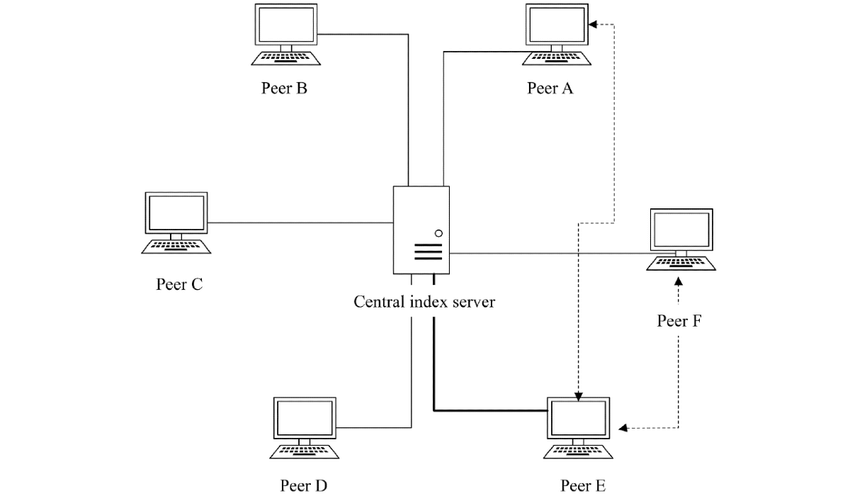
\includegraphics[width = 0.5\textwidth]{Imagenes/Vectorial/p2p_centralized}
    \caption{Ejemplo de arquitectura P2P centralizada}
    \label{fig:p2pcentralized}
\end{figure}


Un ejemplo representativo de este modelo es Napster, una de las primeras aplicaciones de intercambio de archivos en redes P2P.
En Napster, los usuarios podían buscar canciones mediante el servidor central, que les proporcionaba una lista de nodos disponibles que poseían el archivo solicitado.
Aunque las transferencias de datos se realizaban directamente entre los nodos, toda la coordinación dependía del servidor central.
Este diseño permitió a Napster ofrecer un servicio rápido y eficiente para la localización de archivos \cite{oram2001}.

Sin embargo, la dependencia de un único punto de control introdujo limitaciones significativas en las redes centralizadas.
La principal desventaja es la vulnerabilidad ante fallos del servidor, ya que su caída puede interrumpir por completo el funcionamiento de la red.
Además, esta arquitectura plantea retos relacionados con la escalabilidad.
A medida que el número de nodos y peticiones aumenta, el servidor central puede convertirse en un cuello de botella, afectando negativamente al rendimiento general del sistema.

Otro problema importante de las arquitecturas centralizadas es su exposición a riesgos legales y regulatorios.
En el caso de Napster, las demandas por infracción de derechos de autor llevaron al cierre de sus servidores en 2001, lo que dejó a los usuarios sin acceso a la red.
Este incidente manifesto la fragilidad de este modelo frente a las presiones externas, fomentando el desarrollo de alternativas más descentralizadas.

A pesar de sus limitaciones, las arquitecturas centralizadas siguen siendo útiles en ciertos escenarios donde la eficiencia y el control son prioritarios.
Por ejemplo, en redes pequeñas o sistemas donde la localización rápida de recursos es más importante que la resiliencia, un enfoque centralizado puede resultar ventajoso.
En estos casos, el servidor actúa como un mediador confiable, garantizando la consistencia y facilitando la gestión de la red.

\subsection{Arquitecturas descentralizadas}

En las redes P2P descentralizadas, todos los nodos participan con el mismo rol, asumiendo tanto funciones de cliente como de servidor.
A diferencia de las arquitecturas centralizadas, estas redes eliminan el servidor único como punto de coordinación, distribuyendo las responsabilidades entre los nodos participantes.
Este diseño aumenta significativamente la resiliencia de la red, ya que no depende de un único punto de fallo para su funcionamiento.

Una de las características distintivas de las arquitecturas descentralizadas es su capacidad para formar redes en malla.
Cada nodo establece conexiones con otros nodos vecinos, permitiendo la transferencia directa de datos sin intermediarios.
Este enfoque mejora la redundancia, ya que incluso si varios nodos fallan, la red puede seguir operando al redirigir las conexiones a través de otros caminos disponibles.
Sin embargo, esta descentralización también introduce nuevos problemas, como la necesidad de algoritmos eficientes para la localización de recursos y la gestión del tráfico de red.

Dentro de las arquitecturas descentralizadas, podemos diferenciar dos tipos principales: \textbf{estructuradas} y \textbf{no estructuradas},
cada una con características, ventajas e inconvenientes.

\subparagraph{Redes no estructuradas}

En las redes no estructuradas, los nodos se conectan de manera arbitraria, sin una organización predefinida en la topología de la red.
Estas redes se basan en conexiones dinámicas entre nodos vecinos, lo que permite la transferencia directa de datos sin intermediarios.
Este diseño mejora la redundancia, la localización de recursos es más compleja.
En estas redes, las búsquedas suelen realizarse mediante técnicas como \textit{flooding} o \textit{broadcast},
donde un nodo envía una solicitud a todos sus vecinos, y estos la retransmiten a los suyos.
Aunque estas técnicas son efectivas en redes pequeñas, generan un gran volumen de tráfico en redes más grandes, afectando significativamente el rendimiento.

La simplicidad de las redes no estructuradas las hace ideales para aplicaciones donde los recursos se distribuyen de manera uniforme y la actividad de los nodos es impredecible.
Sin embargo, no garantizan que un recurso disponible sea localizado con éxito, especialmente en redes heterogéneas y de gran escala.
Las primeras versiones de Gnutella son un ejemplo clásico de esta arquitectura, donde cada nodo actuaba de forma completamente autónoma sin una estructura definida.

\subparagraph{Redes estructuradas}

Por otro lado, las redes estructuradas imponen una organización específica sobre la topología de la red, lo que las hace más eficientes para la localización de recursos.
Estas redes utilizan algoritmos distribuidos para asignar identificadores únicos a nodos y recursos,
creando un espacio lógico donde la ubicación de cualquier recurso puede ser calculada de manera predecible.
Las tablas hash distribuidas (DHTs) son un ejemplo común de este enfoque.

En las redes estructuradas, como Chord, cada nodo y recurso se asigna a una posición dentro de un anillo lógico basado en una función hash.
Esto permite realizar búsquedas con una complejidad logarítmica, en lugar de depender de técnicas de \textit{flooding}.
Esta organización mejora la escalabilidad y la eficiencia de las redes, haciéndolas ideales para aplicaciones donde se requiere una alta predictibilidad en la localización de datos.

Aunque las redes estructuradas ofrecen claras ventajas en términos de eficiencia, también tienen algunas limitaciones.
Su implementación es más compleja y requiere que los nodos sigan estrictamente las reglas del protocolo para mantener la integridad de la red.
Además, son más vulnerables a nodos maliciosos que podrían intentar alterar la topología de la red o la asignación de recursos.

\subparagraph{Comparación y aplicaciones actuales}

Tanto las redes no estructuradas como las estructuradas tienen ventajas y desventajas que las hacen adecuadas para diferentes aplicaciones.
Las redes no estructuradas son mejores en su flexibilidad y simplicidad, lo que las hace útiles en aplicaciones donde no se requiere una localización precisa de recursos.
Por otro lado, las redes estructuradas son preferidas en sistemas donde la eficiencia y la predictibilidad son críticas,
como en aplicaciones de almacenamiento distribuido como BitTorrent.

En la actualidad, muchas arquitecturas descentralizadas han evolucionado hacia modelos híbridos, combinando elementos de ambos enfoques.
Por ejemplo, el uso de supernodos en redes no estructuradas mejora la eficiencia al centralizar parcialmente ciertas funciones,
mientras que las DHTs han sido integradas en sistemas más flexibles para manejar fallos de nodos o entornos más dinámicos.


\subsection{Arquitecturas híbridas}

Las arquitecturas híbridas combinan elementos de las arquitecturas centralizadas y descentralizadas, logrando un equilibrio entre eficiencia, escalabilidad y resiliencia.
Este enfoque es común en redes que requieren una coordinación inicial centralizada para algunas tareas, mientras mantienen la descentralización en la transferencia de datos.
Este diseño aprovecha la simplicidad de las centralizadas y la flexibilidad de las descentralizadas.

Las redes híbridas suelen tener un servidor central o un conjunto de nodos especializados que gestionan funciones como la indexación de recursos,
la localización de nodos o la autenticación de usuarios.
Sin embargo, la transferencia de datos se hace de manera descentralizada, lo que permite que la red continúe funcionando incluso si los nodos centralizados fallan.

\paragraph{BitTorrent} es el ejemplo más popular de una arquitectura híbrida que combina características de ambos tipos de redes.
En su implementación clásica, utiliza trackers, servidores centralizados que ayudan en la localización inicial de recursos.
Estos trackers proporcionan una lista de peers (nodos) que poseen partes del archivo solicitado, facilitando el inicio de las transferencias.

El diseño híbrido de BitTorrent se basa en dos componentes:
\begin{itemize}
    \item \textbf{Tracker centralizado:} Los trackers centralizados actúan como mediadores para localizar recursos.
    Aunque no participan directamente en la transferencia de datos, son esenciales para la localización de los peers.
    \item \textbf{Transferencia descentralizada:} Una vez que el tracker proporciona la información sobre los peers, la transferencia de datos se realiza directamente entre los nodos, utilizando una estructura completamente descentralizada.
\end{itemize}

La combinación de estos dos elementos permite a BitTorrent equilibrar eficiencia y escalabilidad.
Sin embargo, la dependencia de trackers introduce vulnerabilidades, como puntos únicos de fallo.
Para mitigar esto, BitTorrent ha evolucionado hacia modelos más descentralizados mediante el uso de Tablas Hash Distribuidas (DHT), que eliminan la necesidad de trackers centrales,
aumentando la robustez de la red.

\section{Protocolos de comunicación en redes P2P}

\subsection{Protocolos de transporte: TCP y UDP}
Los protocolos TCP (Transmission Control Protocol) y UDP (User Datagram Protocol) son los más usados para la comunicación de nodos en redes P2P.
Aunque ambos son esenciales para la transmisión de datos entre nodos, tienen diferencias fundamentales que los hacen más adecuados para algunos tipos aplicaciones específicas.
TCP prioriza la fiabilidad y la entrega ordenada de los datos, mientras que UDP, es más rápido y ligero, por lo que es mejor para aplicaciones que necesitan menor latencia.
En las siguientes secciones, se analizarán las características de ambos protocolos.


\subsubsection{Protocolo TCP}
El Transmission Control Protocol (TCP) es uno de los pilares fundamentales en las comunicaciones de redes Peer-to-Peer (P2P). Este protocolo de transporte confiable garantiza la entrega íntegra y ordenada de los datos entre dos nodos, lo que lo convierte en una herramienta clave para aplicaciones que priorizan la fiabilidad. TCP opera en un modelo orientado a la conexión, lo que implica que antes de transferir datos, se debe establecer una conexión entre los nodos implicados. Estas características hacen que TCP sea especialmente útil en redes P2P, incluso en entornos con condiciones de red variables.

\subsubsection*{Establecimiento de conexión: Three-Way Handshake}
El proceso de inicialización en TCP, conocido como Three-Way Handshake, permite establecer una conexión confiable entre dos nodos. Este procedimiento consta de tres pasos principales:

\begin{enumerate}
\item SYN: El nodo que inicia la conexión envía un paquete de sincronización (SYN) al nodo receptor, indicando su intención de establecer comunicación.
\item SYN-ACK: El receptor responde con un paquete de sincronización y acuse de recibo (SYN-ACK), confirmando la recepción del mensaje inicial y mostrando su disposición para continuar.
\item ACK: Finalmente, el nodo iniciador envía un paquete de acuse de recibo (ACK), completando el proceso y estableciendo la conexión.
\end{enumerate}
Este mecanismo permite a ambos nodos acordar parámetros fundamentales, como los números de secuencia iniciales y las ventanas de transmisión. Estos parámetros son esenciales para garantizar la sincronización durante la transmisión y la integridad de los datos \cite{stevens1994tcp}.

\subsubsection*{Mecanismos de fiabilidad}
TCP incluye varios mecanismos diseñados para garantizar que los datos lleguen correctamente al destino, incluso en presencia de fallos en la red:

\begin{itemize}
\item Números de secuencia: Cada byte transmitido está asociado a un número de secuencia único, que permite identificar el orden correcto de los datos y detectar duplicados.
\item Acuse de recibo (ACK): El receptor confirma la recepción de los datos enviando un mensaje ACK al emisor, indicando el próximo byte esperado. Este sistema asegura que los segmentos recibidos sean correctamente identificados.
\item Retransmisión de paquetes: Si el emisor no recibe un acuse de recibo dentro de un tiempo específico calculado dinámicamente (Retransmission Timeout, RTO), el paquete se retransmite \cite{jacobson1988congestion}.
\item Checksum: Cada segmento contiene un valor checksum que valida la integridad de los datos. Si el checksum recibido no coincide, el segmento se descarta \cite{kurose2016computer}.
\end{itemize}
Estos mecanismos garantizan la fiabilidad y precisión en la transmisión, una característica esencial para aplicaciones de intercambio de archivos en redes P2P.

\subsubsection*{Control de flujo y congestión}
Para gestionar la transferencia de datos de manera eficiente, TCP utiliza algoritmos avanzados de control de flujo y congestión:

\begin{itemize}
\item Ventana deslizante (Sliding Window Protocol): Este sistema permite al emisor transmitir múltiples segmentos sin esperar confirmación individual para cada uno, optimizando el uso del ancho de banda disponible.
\item Control de congestión: TCP adapta dinámicamente su tasa de transmisión según las condiciones de la red. Los principales algoritmos utilizados incluyen:\begin{itemize}
\item Slow Start: Inicia con un tamaño de ventana reducido, que aumenta exponencialmente hasta que se detectan signos de congestión.
\item Congestion Avoidance: Tras alcanzar la capacidad de la red, el crecimiento del tamaño de la ventana es lineal.
\item Fast Retransmit: Cuando se detectan tres ACK duplicados consecutivos, TCP asume que un paquete se perdió y lo retransmite inmediatamente, sin esperar al tiempo de retransmisión (RTO) \cite{jacobson1988congestion}.
\end{itemize}

\end{itemize}
Estos mecanismos permiten que TCP maximice el rendimiento, evitando la saturación de la red y garantizando una transferencia fluida.

\subsubsection*{Desafíos de TCP en redes P2P}
A pesar de sus ventajas, TCP enfrenta ciertos desafíos en el contexto de redes P2P:

\begin{enumerate}
\item Overhead en la gestión de conexiones: Cada conexión TCP requiere recursos significativos, como memoria y capacidad de procesamiento. En redes P2P, donde los nodos deben establecer y mantener múltiples conexiones simultáneamente, este overhead puede limitar el rendimiento \cite{cohen2003}.
\item Latencia: Los mecanismos de retransmisión y control de flujo pueden introducir retrasos, especialmente en redes congestionadas o de alta latencia.
\item Escalabilidad: La necesidad de gestionar múltiples conexiones persistentes puede convertirse en un cuello de botella en sistemas con miles de nodos.
\end{enumerate}
\subsubsection*{Relevancia de TCP en redes P2P}
A pesar de estos desafíos, TCP sigue siendo el protocolo dominante para aplicaciones P2P que priorizan la fiabilidad y la integridad de los datos. Sistemas como BitTorrent utilizan TCP para transferir fragmentos de archivos entre nodos, asegurando que cada parte se reciba de manera correcta antes de ensamblar el archivo completo. Su capacidad para operar en redes heterogéneas y manejar errores lo convierte en una herramienta esencial en el diseño de redes P2P modernas \cite{cohen2003}.


\subsubsection{Protocolo UDP}

\subsection{Configuración y gestión de conectividad en redes P2P}
\subsubsection{Problemas de NAT y firewalls}
\subsubsection{Configuración automática mediante UPnP}
\subsubsection{STUN y TURN como soluciones para NAT traversal}

\chapter{Diseno y desarrollo de la aplicaci\'on}
\label{cap:descripcionTrabajo}

3.1. Diseño del sistema
3.1.1. Arquitectura general
3.1.2. Módulos principales del sistema
3.2. Desarrollo del cliente con interfaz gráfica
3.2.1. Funcionalidades implementadas
3.2.2. Desafíos técnicos y soluciones aplicadas
3.3. Sistema de registro y gestión de nodos
3.3.1. Diseño e implementación
3.3.2. Pruebas funcionales
3.4. Comunicación entre nodos
3.4.1. Protocolo basado en TCP
3.4.2. Integración con el cliente
3.5. Integración del soporte para UPnP
3.5.1. Automatización de configuración de puertos
3.5.2. Validación en diferentes entornos de red
3.6. Evaluación del sistema
3.6.1. Pruebas realizadas y resultados
3.6.2. Análisis de los resultados

%\include{Capitulos/Capitulo4}
%\include{Capitulos/Capitulo5}
\chapter{Conclusiones y Trabajo Futuro}
\label{cap:conclusiones}

Conclusiones del trabajo y líneas de trabajo futuro.

Antes de la entrega de actas de cada convocatoria, en el plazo que se indica en el calendario de los trabajos de fin de máster, el estudiante entregará en el Campus Virtual la versión final de la memoria en PDF. En la portada de la misma deberán figurar, como se ha señalado anteriormente, la convocatoria y la calificación obtenida. Asimismo, el estudiante también entregará todo el material que tenga concedido en préstamo a lo largo del curso.




%%%%%%%%%%%%%%%%%%%%%%%%%%%%%%%%%%%%%%%%%%%%%%%%%%%%%%%%%%%%%%%%%%%%%%%%%%%
% Si el TFM se escribe en inglés, comentar las siguientes líneas 
% porque no es necesario incluir nuevamente las Conclusiones en inglés
\begin{otherlanguage}{english}
\chapter{Introduction}
\label{cap:introduction}

Introduction to the subject area. This chapter contains the translation of Chapter \ref{cap:introduccion}.










\chapter{Conclusions and Future Work}
\label{cap:conclusions}

Conclusions and future lines of work. This chapter contains the translation of Chapter \ref{cap:conclusiones}.



\end{otherlanguage}
%%%%%%%%%%%%%%%%%%%%%%%%%%%%%%%%%%%%%%%%%%%%%%%%%%%%%%%%%%%%%%%%%%%%%%%%%%%

%
% Bibliografía
%
% Si el TFM se escribe en inglés, editar TeXiS/TeXiS_bib para cambiar el
% estilo de las referencias
%---------------------------------------------------------------------
%
%                      configBibliografia.tex
%
%---------------------------------------------------------------------
%
% bibliografia.tex
% Copyright 2009 Marco Antonio Gomez-Martin, Pedro Pablo Gomez-Martin
%
% This file belongs to the TeXiS manual, a LaTeX template for writting
% Thesis and other documents. The complete last TeXiS package can
% be obtained from http://gaia.fdi.ucm.es/projects/texis/
%
% Although the TeXiS template itself is distributed under the 
% conditions of the LaTeX Project Public License
% (http://www.latex-project.org/lppl.txt), the manual content
% uses the CC-BY-SA license that stays that you are free:
%
%    - to share & to copy, distribute and transmit the work
%    - to remix and to adapt the work
%
% under the following conditions:
%
%    - Attribution: you must attribute the work in the manner
%      specified by the author or licensor (but not in any way that
%      suggests that they endorse you or your use of the work).
%    - Share Alike: if you alter, transform, or build upon this
%      work, you may distribute the resulting work only under the
%      same, similar or a compatible license.
%
% The complete license is available in
% http://creativecommons.org/licenses/by-sa/3.0/legalcode
%
%---------------------------------------------------------------------
%
% Fichero  que  configura  los  parámetros  de  la  generación  de  la
% bibliografía.  Existen dos  parámetros configurables:  los ficheros
% .bib que se utilizan y la frase célebre que aparece justo antes de la
% primera referencia.
%
%---------------------------------------------------------------------


%%%%%%%%%%%%%%%%%%%%%%%%%%%%%%%%%%%%%%%%%%%%%%%%%%%%%%%%%%%%%%%%%%%%%%
% Definición de los ficheros .bib utilizados:
% \setBibFiles{<lista ficheros sin extension, separados por comas>}
% Nota:
% Es IMPORTANTE que los ficheros estén en la misma línea que
% el comando \setBibFiles. Si se desea utilizar varias líneas,
% terminarlas con una apertura de comentario.
%%%%%%%%%%%%%%%%%%%%%%%%%%%%%%%%%%%%%%%%%%%%%%%%%%%%%%%%%%%%%%%%%%%%%%
\setBibFiles{%
biblio%
}

%%%%%%%%%%%%%%%%%%%%%%%%%%%%%%%%%%%%%%%%%%%%%%%%%%%%%%%%%%%%%%%%%%%%%%
% Definición de la frase célebre para el capítulo de la
% bibliografía. Dentro normalmente se querrá hacer uso del entorno
% \begin{FraseCelebre}, que contendrá a su vez otros dos entornos,
% un \begin{Frase} y un \begin{Fuente}.
%
% Nota:
% Si no se quiere cita, se puede eliminar su definición (en la
% macro setCitaBibliografia{} ).
%%%%%%%%%%%%%%%%%%%%%%%%%%%%%%%%%%%%%%%%%%%%%%%%%%%%%%%%%%%%%%%%%%%%%%
\setCitaBibliografia{
\begin{FraseCelebre}
\begin{Frase}
  Y así, del mucho leer y del poco dormir, se le secó el celebro de
  manera que vino a perder el juicio.\\ 
  \textcolor{red}{(modificar en Cascaras$\backslash$bibliografia.tex)}
\end{Frase}
\begin{Fuente}
  Miguel de Cervantes Saavedra
\end{Fuente}
\end{FraseCelebre}
}

%%
%% Creamos la bibliografia
%%
\makeBib

% Variable local para emacs, para  que encuentre el fichero maestro de
% compilación y funcionen mejor algunas teclas rápidas de AucTeX

%%%
%%% Local Variables:
%%% mode: latex
%%% TeX-master: "../Tesis.tex"
%%% End:



% Apéndices
\appendix
\chapter{Título del Apéndice A}
\label{Appendix:Key1}

Contenido del apéndice
\chapter{Título del Apéndice B}
\label{Appendix:Key2}

%\include{Apendices/appendixC}
%\include{...}
%\include{...}
%\include{...}
\backmatter



%
% Índice de palabras
%

% Sólo  la   generamos  si  está   declarada  \generaindice.  Consulta
% TeXiS.sty para más información.

% En realidad, el soporte para la generación de índices de palabras
% en TeXiS no está documentada en el manual, porque no ha sido usada
% "en producción". Por tanto, el fichero que genera el índice
% *no* se incluye aquí (está comentado). Consulta la documentación
% en TeXiS_pream.tex para más información.
\ifx\generaindice\undefined
\else
%%---------------------------------------------------------------------
%
%                        TeXiS_indice.tex
%
%---------------------------------------------------------------------
%
% TeXiS_indice.tex
% Copyright 2009 Marco Antonio Gomez-Martin, Pedro Pablo Gomez-Martin
%
% This file belongs to TeXiS, a LaTeX template for writting
% Thesis and other documents. The complete last TeXiS package can
% be obtained from http://gaia.fdi.ucm.es/projects/texis/
%
% This work may be distributed and/or modified under the
% conditions of the LaTeX Project Public License, either version 1.3
% of this license or (at your option) any later version.
% The latest version of this license is in
%   http://www.latex-project.org/lppl.txt
% and version 1.3 or later is part of all distributions of LaTeX
% version 2005/12/01 or later.
%
% This work has the LPPL maintenance status `maintained'.
% 
% The Current Maintainers of this work are Marco Antonio Gomez-Martin
% and Pedro Pablo Gomez-Martin
%
%---------------------------------------------------------------------
%
% Contiene  los  comandos  para  generar  el índice  de  palabras  del
% documento.
%
%---------------------------------------------------------------------
%
% NOTA IMPORTANTE: el  soporte en TeXiS para el  índice de palabras es
% embrionario, y  de hecho  ni siquiera se  describe en el  manual. Se
% proporciona  una infraestructura  básica (sin  terminar)  para ello,
% pero  no ha  sido usada  "en producción".  De hecho,  a pesar  de la
% existencia de  este fichero, *no* se incluye  en Tesis.tex. Consulta
% la documentación en TeXiS_pream.tex para más información.
%
%---------------------------------------------------------------------


% Si se  va a generar  la tabla de  contenidos (el índice  habitual) y
% también vamos a  generar el índice de palabras  (ambas decisiones se
% toman en  función de  la definición  o no de  un par  de constantes,
% puedes consultar modo.tex para más información), entonces metemos en
% la tabla de contenidos una  entrada para marcar la página donde está
% el índice de palabras.

\ifx\generatoc\undefined
\else
   \addcontentsline{toc}{chapter}{\indexname}
\fi


% Generamos el índice
\printindex

% Variable local para emacs, para  que encuentre el fichero maestro de
% compilación y funcionen mejor algunas teclas rápidas de AucTeX

%%%
%%% Local Variables:
%%% mode: latex
%%% TeX-master: "./tesis.tex"
%%% End:

\fi

%
% Lista de acrónimos
%

% Sólo  lo  generamos  si  está declarada  \generaacronimos.  Consulta
% TeXiS.sty para más información.


\ifx\generaacronimos\undefined
\else
%---------------------------------------------------------------------
%
%                        TeXiS_acron.tex
%
%---------------------------------------------------------------------
%
% TeXiS_acron.tex
% Copyright 2009 Marco Antonio Gomez-Martin, Pedro Pablo Gomez-Martin
%
% This file belongs to TeXiS, a LaTeX template for writting
% Thesis and other documents. The complete last TeXiS package can
% be obtained from http://gaia.fdi.ucm.es/projects/texis/
%
% This work may be distributed and/or modified under the
% conditions of the LaTeX Project Public License, either version 1.3
% of this license or (at your option) any later version.
% The latest version of this license is in
%   http://www.latex-project.org/lppl.txt
% and version 1.3 or later is part of all distributions of LaTeX
% version 2005/12/01 or later.
%
% This work has the LPPL maintenance status `maintained'.
% 
% The Current Maintainers of this work are Marco Antonio Gomez-Martin
% and Pedro Pablo Gomez-Martin
%
%---------------------------------------------------------------------
%
% Contiene  los  comandos  para  generar  el listado de acrónimos
% documento.
%
%---------------------------------------------------------------------
%
% NOTA IMPORTANTE:  para que la  generación de acrónimos  funcione, al
% menos  debe  existir  un  acrónimo   en  el  documento.  Si  no,  la
% compilación  del   fichero  LaTeX  falla  con   un  error  "extraño"
% (indicando  que  quizá  falte  un \item).   Consulta  el  comentario
% referente al paquete glosstex en TeXiS_pream.tex.
%
%---------------------------------------------------------------------


% Redefinimos a español  el título de la lista  de acrónimos (Babel no
% lo hace por nosotros esta vez)

\def\listacronymname{Lista de acrónimos}

% Para el glosario:
% \def\glosarryname{Glosario}

% Si se  va a generar  la tabla de  contenidos (el índice  habitual) y
% también vamos a  generar la lista de acrónimos  (ambas decisiones se
% toman en  función de  la definición  o no de  un par  de constantes,
% puedes consultar config.tex  para más información), entonces metemos
% en la  tabla de contenidos una  entrada para marcar  la página donde
% está el índice de palabras.

\ifx\generatoc\undefined
\else
   \addcontentsline{toc}{chapter}{\listacronymname}
\fi


% Generamos la lista de acrónimos (en realidad el índice asociado a la
% lista "acr" de GlossTeX)

\printglosstex(acr)

% Variable local para emacs, para  que encuentre el fichero maestro de
% compilación y funcionen mejor algunas teclas rápidas de AucTeX

%%%
%%% Local Variables:
%%% mode: latex
%%% TeX-master: "../Tesis.tex"
%%% End:

\fi

%
% Final
%
%\end{otherlanguage}
\end{document}
